% A distance to the closed interval, illustrated with numeric representative positions.
\begin{center}
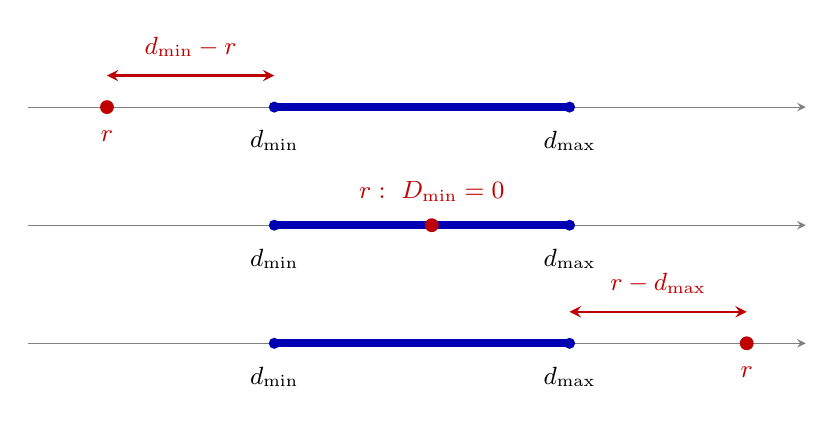
\begin{tikzpicture}[x=1.25cm,y=1cm,font=\small,>=stealth]
\foreach \yy in {0,-1.5,-3} {
 \draw[->,gray] (-.5,\yy)--(7.4,\yy);
 \draw[blue!70!black,line width=3pt] (2,\yy)--(5,\yy);
 \fill[blue!70!black] (2,\yy) circle(2pt) (5,\yy) circle(2pt);
 \node[below=5pt] at (2,\yy) {$d_{\min}$};
 \node[below=5pt] at (5,\yy) {$d_{\max}$};
}
\fill[red!75!black] (.3,0) circle(2.5pt) node[below=5pt] {$r$};
\draw[<->,red!75!black,thick] (.3,.4)--(2,.4) node[midway,above=3pt] {$d_{\min}-r$};
\fill[red!75!black] (3.6,-1.5) circle(2.5pt) node[above=5pt] {$r:\ D_{\min}=0$};
\fill[red!75!black] (6.8,-3) circle(2.5pt) node[below=5pt] {$r$};
\draw[<->,red!75!black,thick] (5,-2.6)--(6.8,-2.6) node[midway,above=3pt] {$r-d_{\max}$};
\end{tikzpicture}
\end{center}
